\label{sec:vnpay-design}
Tích hợp VNPay sử dụng ba thành phần: frontend hiển thị QR/liên kết và trạng thái; NestJS tạo yêu cầu, kiểm chứng kết quả và ghi sổ; VNPay Sandbox xử lý phiên thanh toán thử. QR chứa URL mở trang VNPay, không phải QR chuyển khoản trực tiếp của ứng dụng ngân hàng. Chữ ký và khóa merchant chỉ được xử lý ở backend. Cách phân biệt Return/IPN và quy tắc tham số được đối chiếu với tài liệu VNPay~\cite{VNPAYPAY,VNPAYFAQ}.

\subsubsection{Phân biệt đơn hàng, lần thanh toán và khoản áp dụng}
\begin{table}[htbp]\centering\small
\begin{tabularx}{\linewidth}{|p{.30\linewidth}|X|}\hline
\textbf{Thực thể} & \textbf{Trách nhiệm}\\\hline
Order & Nghĩa vụ phục vụ và tiền còn cần thu: total trừ creditApplied. Một đơn có thể thử thanh toán nhiều lần.\\\hline
VnpayAttempt & Mỗi lần giao dịch có txnRef duy nhất, số tiền, URL, hạn, mã giao dịch nhà cung cấp và trạng thái riêng; giữ lịch sử cả lần thất bại/chưa rõ.\\\hline
PaymentStartRequest & Ánh xạ cặp khách/key tới attempt để gửi lại yêu cầu không tạo thêm lần thanh toán. Key mới vẫn có thể tái dùng mã đang hiệu lực.\\\hline
Payment & Khoản đã xác minh và áp dụng vào Order; không tạo cho mọi attempt hoặc tiền thu nhưng không thể phục vụ. Liên kết attempt duy nhất chống ghi nhận lại cùng lần.\\\hline
PaymentAudit & Nhật ký tạo mã, tra cứu, nhận kết quả và thao tác hỗ trợ; phục vụ truy vết theo attempt, actor và thời gian.\\\hline
PaymentRefundCase & Hồ sơ khoản đã thu nhưng không áp dụng được (thu trùng, đơn không còn hiệu lực); một hồ sơ theo attempt, quầy xử lý bằng chứng từ.\\\hline
\end{tabularx}\caption{Phân tách dữ liệu thanh toán để bảo toàn lịch sử và tránh ghi nhận trùng}
\end{table}

Ví dụ đơn 75.000đ đã chuyển credit 45.000đ chỉ cần thu thêm 30.000đ. Backend ký đúng phần còn thu; frontend không tự quyết định số tiền. Nếu lần A hết hạn rồi cấp B và cả hai cùng thu thành công, chỉ một khoản được áp dụng cho đơn; khoản còn lại có attempt và hồ sơ xử lý riêng, không tạo hai đơn pha chế.

\subsubsection{Luồng và các nhánh kết quả}
Backend kiểm chủ đơn, PENDING/PAYMENT\_FAILED, deadline và snapshot chưa hoàn trước khi cấp mã. Lần mới có txnRef riêng; amount lưu VND nguyên, trường vnp\_Amount gửi sang cổng nhân 100 theo giao thức. Các trường được chuẩn hóa và ký HMAC-SHA512. Hạn QR bị giới hạn bởi deadline giữ món đã trình bày ở mục~\ref{sec:inventory-demand}.

Return xác minh chữ ký, merchant, tham chiếu và số tiền rồi trả HTTP 303 về trang Order; không chuyển PAID. IPN là thông báo server-to-server; QueryDr là truy vấn backend chủ động khi cần kiểm tra. Cả hai kết quả đã xác minh được quy về apply để cùng kiểm soát ghi nhận. Mất Return hoặc khách đóng tab không xóa kết quả đã commit.

\begin{table}[htbp]\centering\small
\begin{tabularx}{\linewidth}{|p{.32\linewidth}|X|}\hline
\textbf{Tình huống} & \textbf{Xử lý trong hệ thống}\\\hline
Thành công, đơn còn đủ điều kiện & Ghi Payment, PAID và điểm trên tiền mới trong cùng transaction; không giữ kho thêm.\\\hline
Thất bại đã xác minh & Ghi FAILED/EXPIRED theo kết quả; đơn còn hạn có thể bắt đầu lần khác.\\\hline
Timeout hoặc kết quả chưa rõ & Giữ lịch sử PENDING/REVIEW, không tự suy ra thất bại. QueryDr chạy ngoài transaction; việc cấp mã mới tuân điều kiện hạn mã/đơn và bằng chứng tiền đã thu.\\\hline
QR hết hạn, đơn còn hạn & Thử tra cứu rồi có thể cấp lần mới dù tra cứu chưa kết luận; giữ attempt cũ để nhận kết quả muộn.\\\hline
IPN lặp hoặc đến ngược thứ tự & Kết quả đã ghi không được ghi lại/cộng điểm lại; thông báo thất bại đến sau không hạ PAID.\\\hline
Thu trùng hoặc tiền về sau khi đơn không còn hiệu lực & Ghi REVIEW và hồ sơ khoản thu không áp dụng; không tự mở lại đơn/pha chế.\\\hline
\end{tabularx}\caption{Quy tắc xử lý kết quả VNPay và thanh toán lại}
\end{table}

\begin{figure}[htbp]\centering
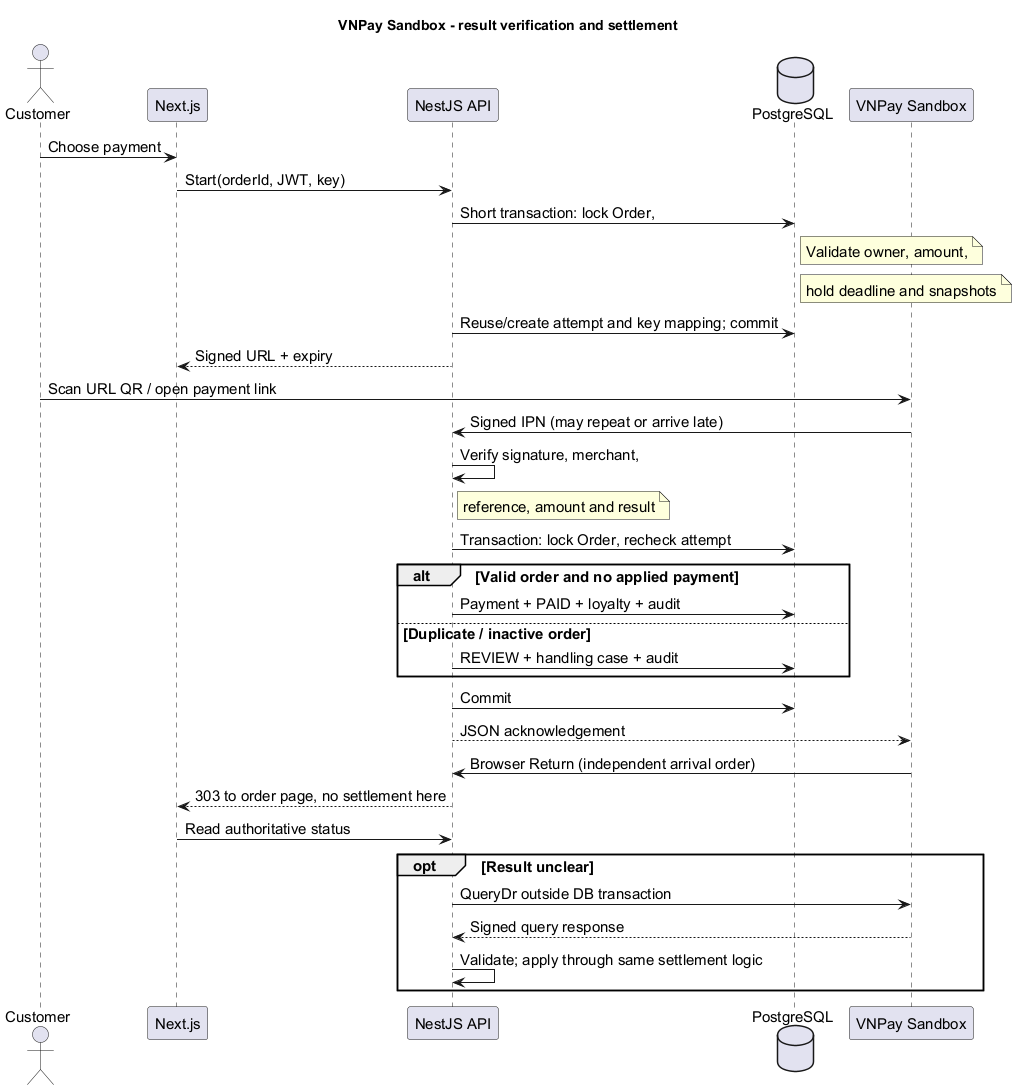
\includegraphics[width=\linewidth,height=.62\textheight,keepaspectratio]{assets/vnpay/vnpay-sequence.png}
\caption{Luồng VNPay: Return điều hướng, IPN/QueryDr xác minh và ghi nhận tại backend}
\end{figure}
